\section{Implementation}

We describes three main components, frontend, scheduler and backend, of the system that serves this model. 

\subsection{Frontend Interface and Features}

We provide two user-facing interfaces tailored for different usage scenarios:

\noindent\textbf{Web-based UI:} A browser-accessible interface for quick demonstration and testing.


\noindent\textbf{Electron App:} A cross-platform desktop application with extended functionalities, including microphone and system audio capture. It supports a floating translation window that remains on top of other applications, making it suitable for use during meetings or media playback.

\begin{figure*}[t]
    \centering
    \begin{minipage}[t]{0.48\textwidth}
        \centering
        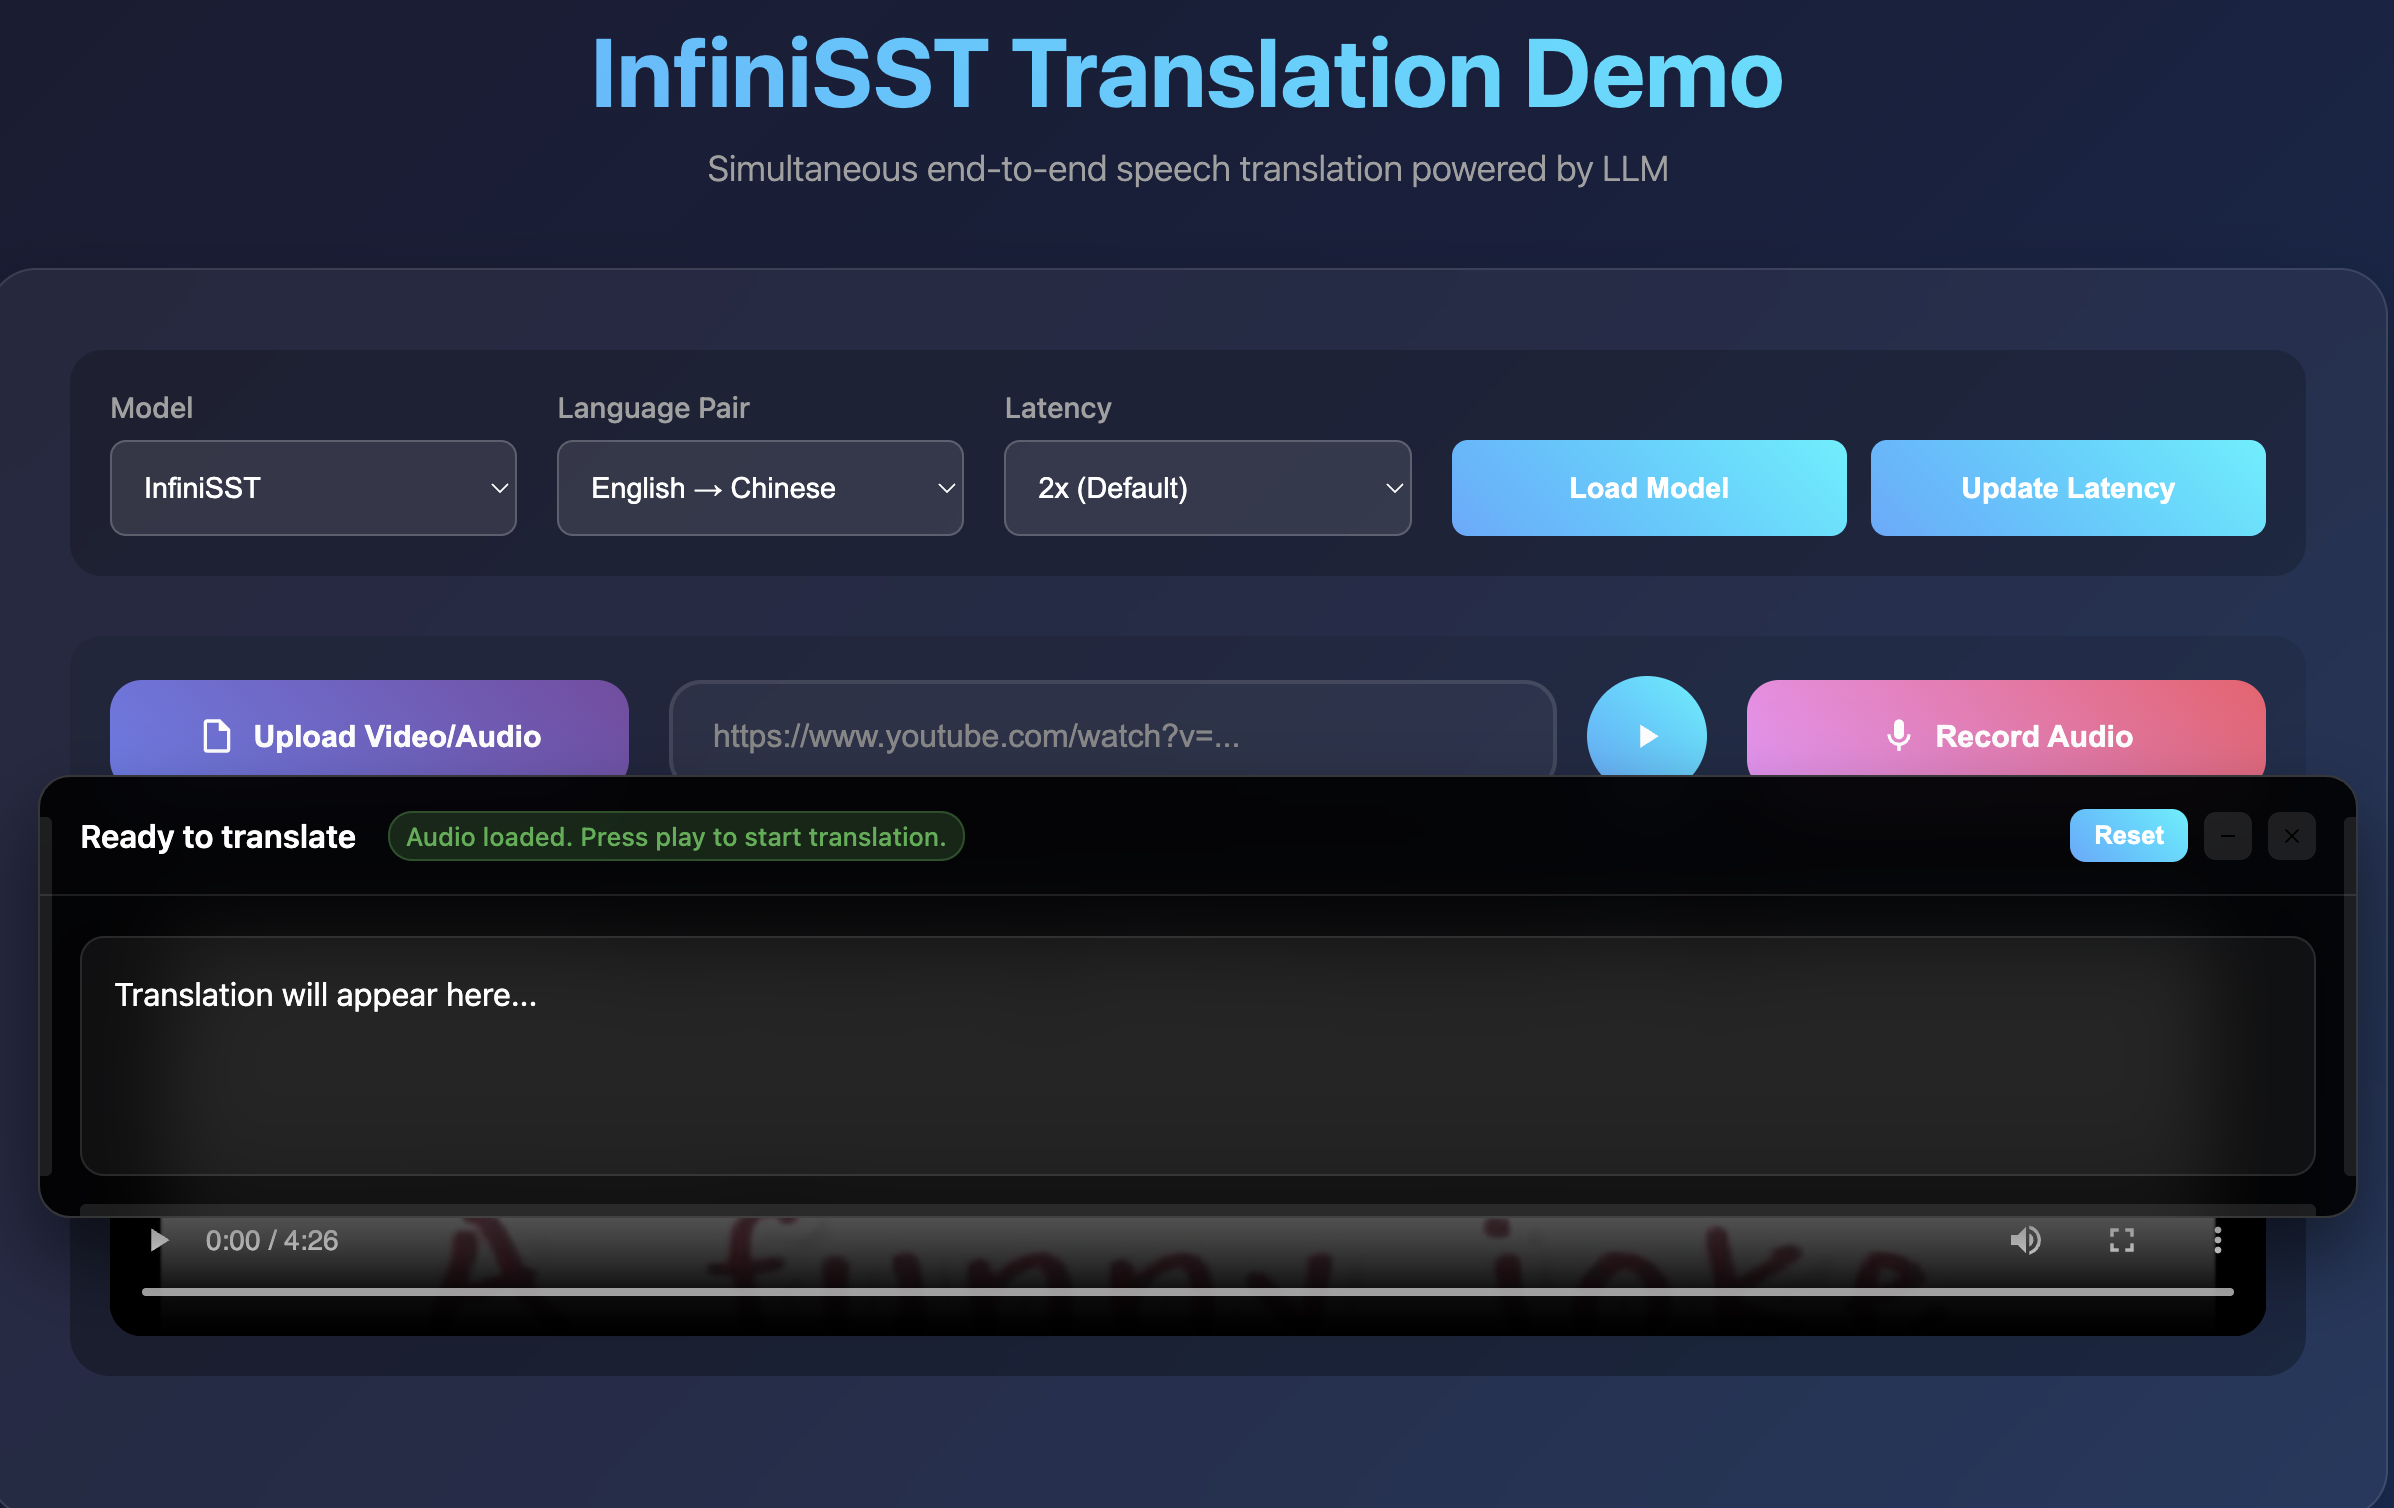
\includegraphics[width=\linewidth]{online.png}
        \caption{Main interface for model selection, latency control, and input configuration.}
        \label{fig:frontend-ui}
    \end{minipage}
    \hfill
    \begin{minipage}[t]{0.48\textwidth}
        \centering
        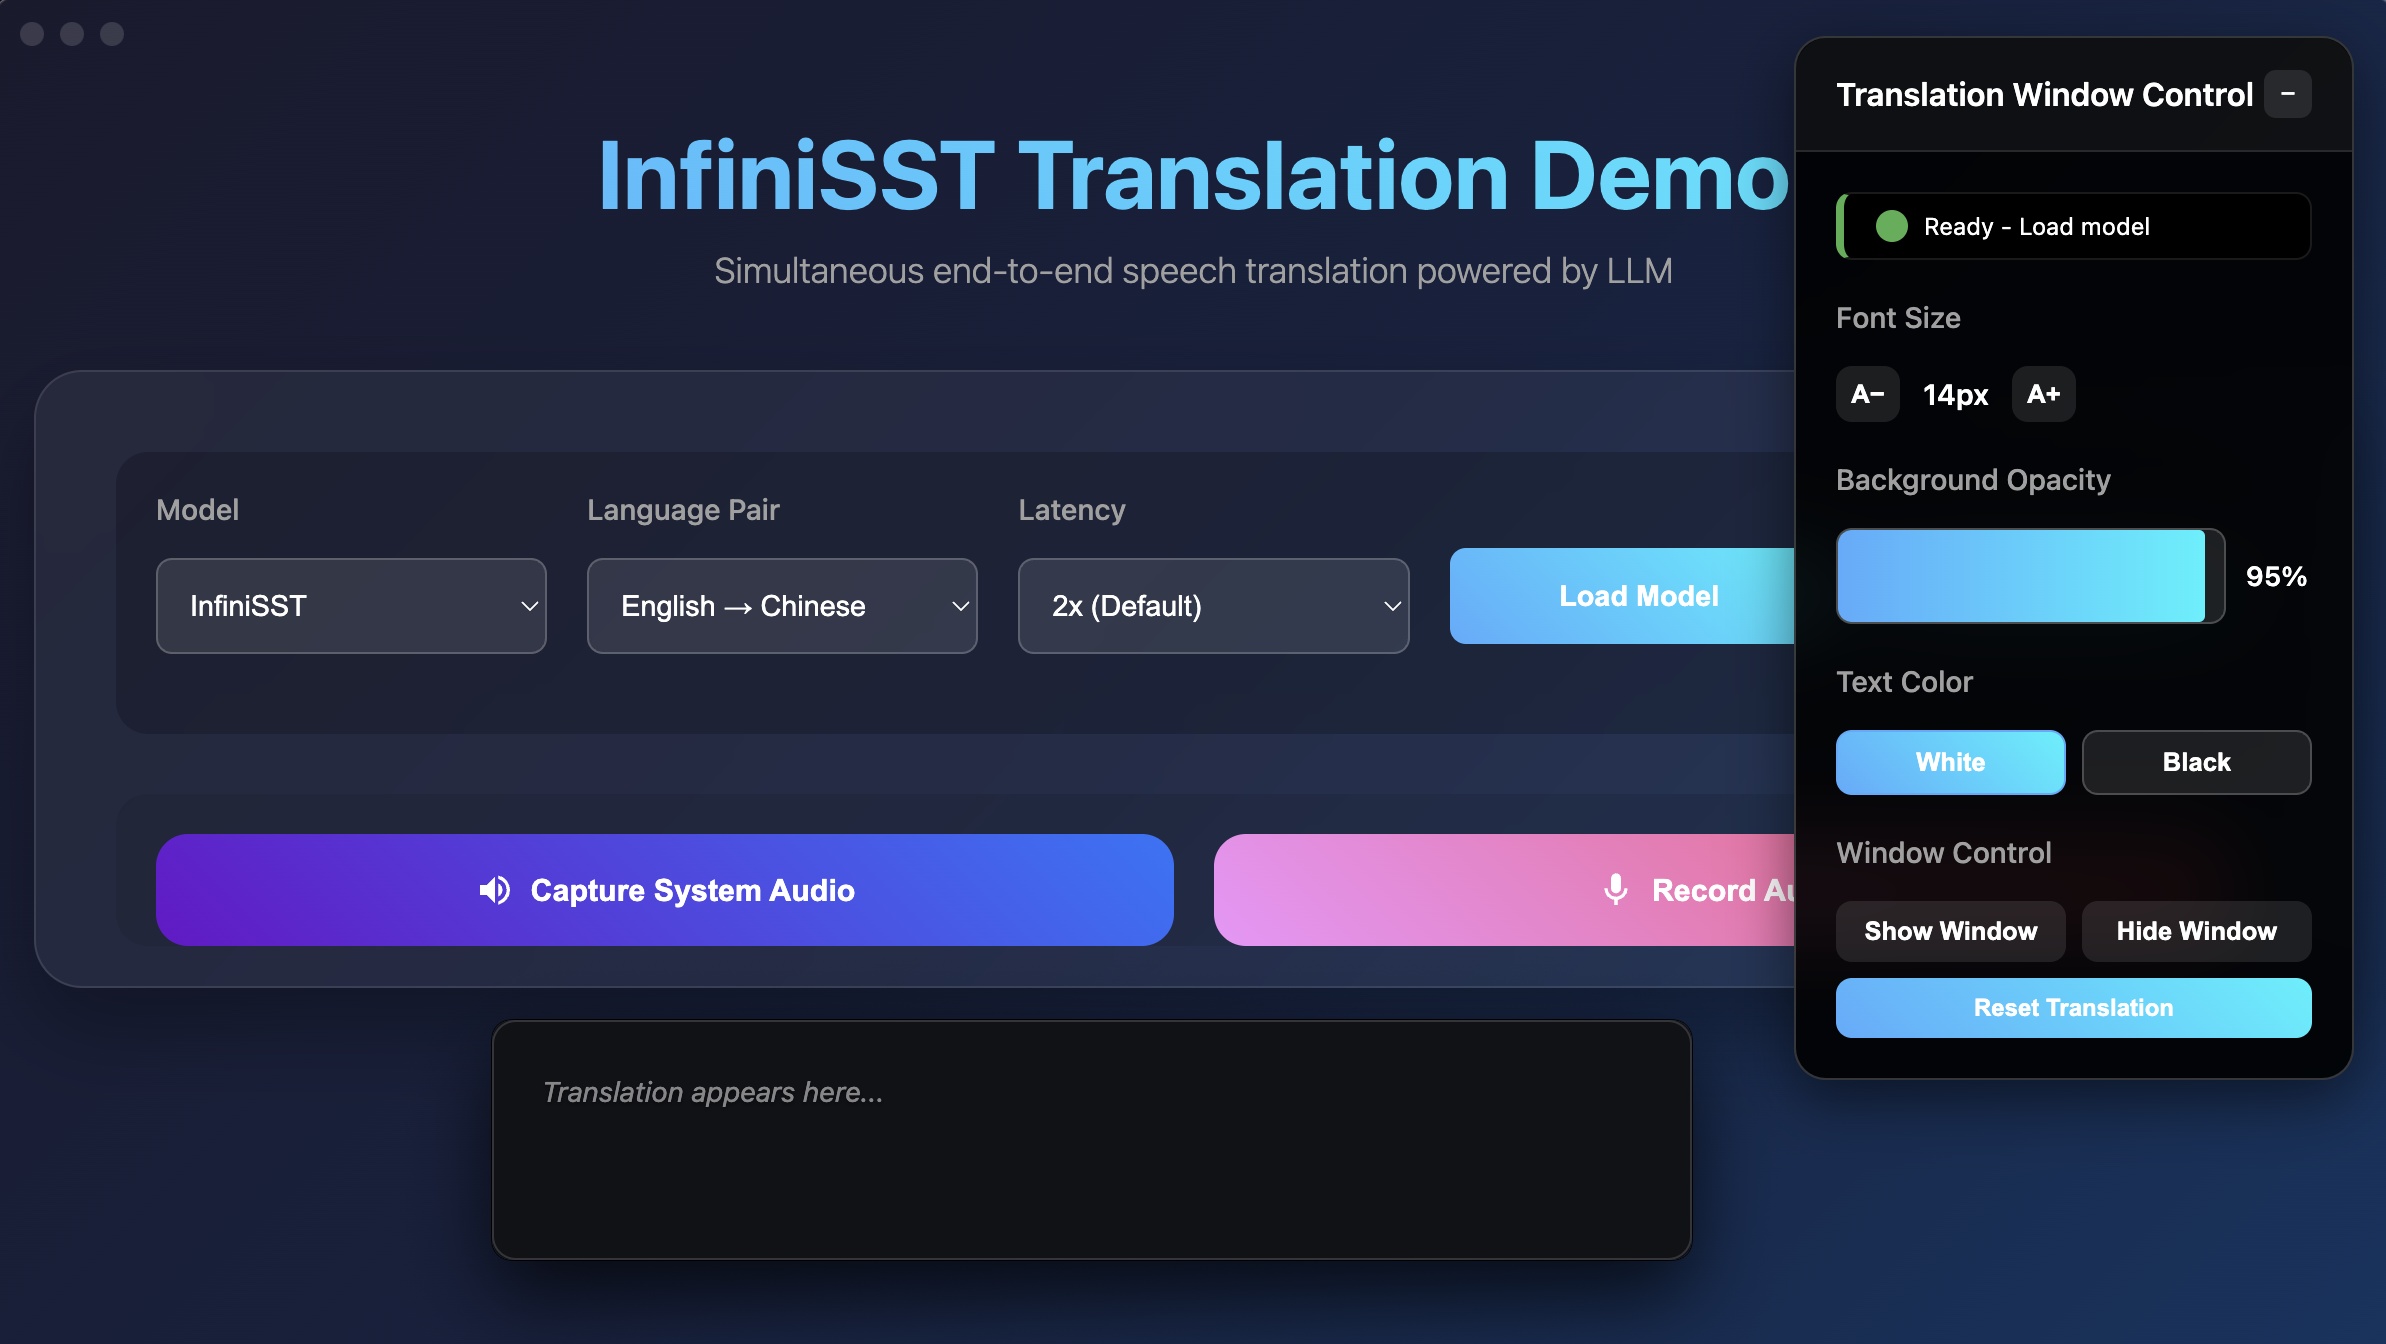
\includegraphics[width=\linewidth]{image_electron.png}
        \caption{Floating translation window for overlay usage during media playback or meetings.}
        \label{fig:floating-window}
    \end{minipage}
\end{figure*}

\noindent\textbf{Audio Input Modalities.}
Our frontend supports four types of audio input to accommodate diverse user needs:
(1) Microphone: captures real-time user speech;
(2) File upload: accepts local audio or video files;
(3) YouTube URL (web version only): processes video content directly from public links;
(4) System audio capture (desktop only): captures system playback audio using tools such as BlackHole on macOS.

\noindent\textbf{User Interface Design.}
The desktop app provides a floating translation window that remains on top of all other applications, enabling users to follow translations while attending meetings or playing media content.

The floating window is highly customizable: users can adjust font size, background opacity, and text color (light/dark mode) in real time. The window supports drag-and-drop repositioning across the screen and can be toggled on or off as needed. A status indicator is included to display session activity, latency level, and streaming status.

A separate control panel allows users to configure translation models, language pairs, and latency settings, offering full control over runtime translation behavior.

\noindent\textbf{Frontend Technology Stack.}
The interface is built with:
Electron (for desktop deployment), HTML/CSS/JavaScript (for UI),
AudioWorklet (for low-latency audio processing),
and WebSocket (for real-time communication with the backend server).

\subsection{LLMScheduler: Concurrency-Aware Scheduling}

The LLMScheduler is designed to coordinate concurrent user sessions efficiently while maintaining low latency and high GPU utilization. Inspired by ORCA-style scheduling, it separates the translation process into two stages---\textit{prefill} and \textit{decode}---each managed by its own dedicated queue.

\paragraph{Queue Management and Locking.}
We maintain two global queues:
(1) a \textbf{prefill queue} for first-token generation or attention resets,
(2) a \textbf{decode queue} for incremental decoding steps.

To reduce contention, we use a \textit{hash-based session-level locking strategy}: each session maps to a lock shard using the hash of its session ID. This enables concurrent scheduling across multiple sessions with minimal lock conflicts. Queue access is protected using non-blocking try-locks to avoid head-of-line blocking and maximize throughput.

Requests within each queue are ordered by arrival time. For translation consistency, we enforce \textbf{intra-session FIFO} ordering and temporarily skip partially processed sessions rather than reorder them.

\paragraph{Dynamic Batch Formation.}
The scheduler forms batches dynamically based on multiple factors:
number of ready requests, waiting time thresholds, session languages, and available model backends. 
This strategy helps:
(i) minimize queuing latency at low traffic;
(ii) fully utilize GPU resources under heavy load;
(iii) adapt to heterogeneous input patterns such as bursty audio or long-form content.

Batch size thresholds are automatically adjusted based on real-time GPU load and traffic conditions.

\paragraph{Session Lifecycle Management.}
Each user session is tracked as a stateful object with fields including session ID, language pair, prefill/decode readiness flags, and last activity timestamp. Sessions are created upon receiving the first valid request and automatically cleaned up after timeout or completion. Associated memory resources (e.g., paged KV cache) are recycled upon destruction.

\paragraph{Scheduling and Prioritization.}
Prefill requests are prioritized over decode to reduce initial response time.
The scheduler ensures:
\begin{itemize}
    \item Session-level order is preserved across batch boundaries
    \item Language-based grouping to avoid cross-model interference
    \item Fair handling of multi-session traffic in concurrent environments
\end{itemize}

\paragraph{Workflow.}
During prefill, the audio encoder output and language model context are used to generate initial tokens. Afterward, decode requests rely on cached KV memory for fast continuation. Both stages maintain consistent state transitions, enabling progressive token emission with correct ordering.
\subsection{Backend}

\begin{figure}
    \centering
    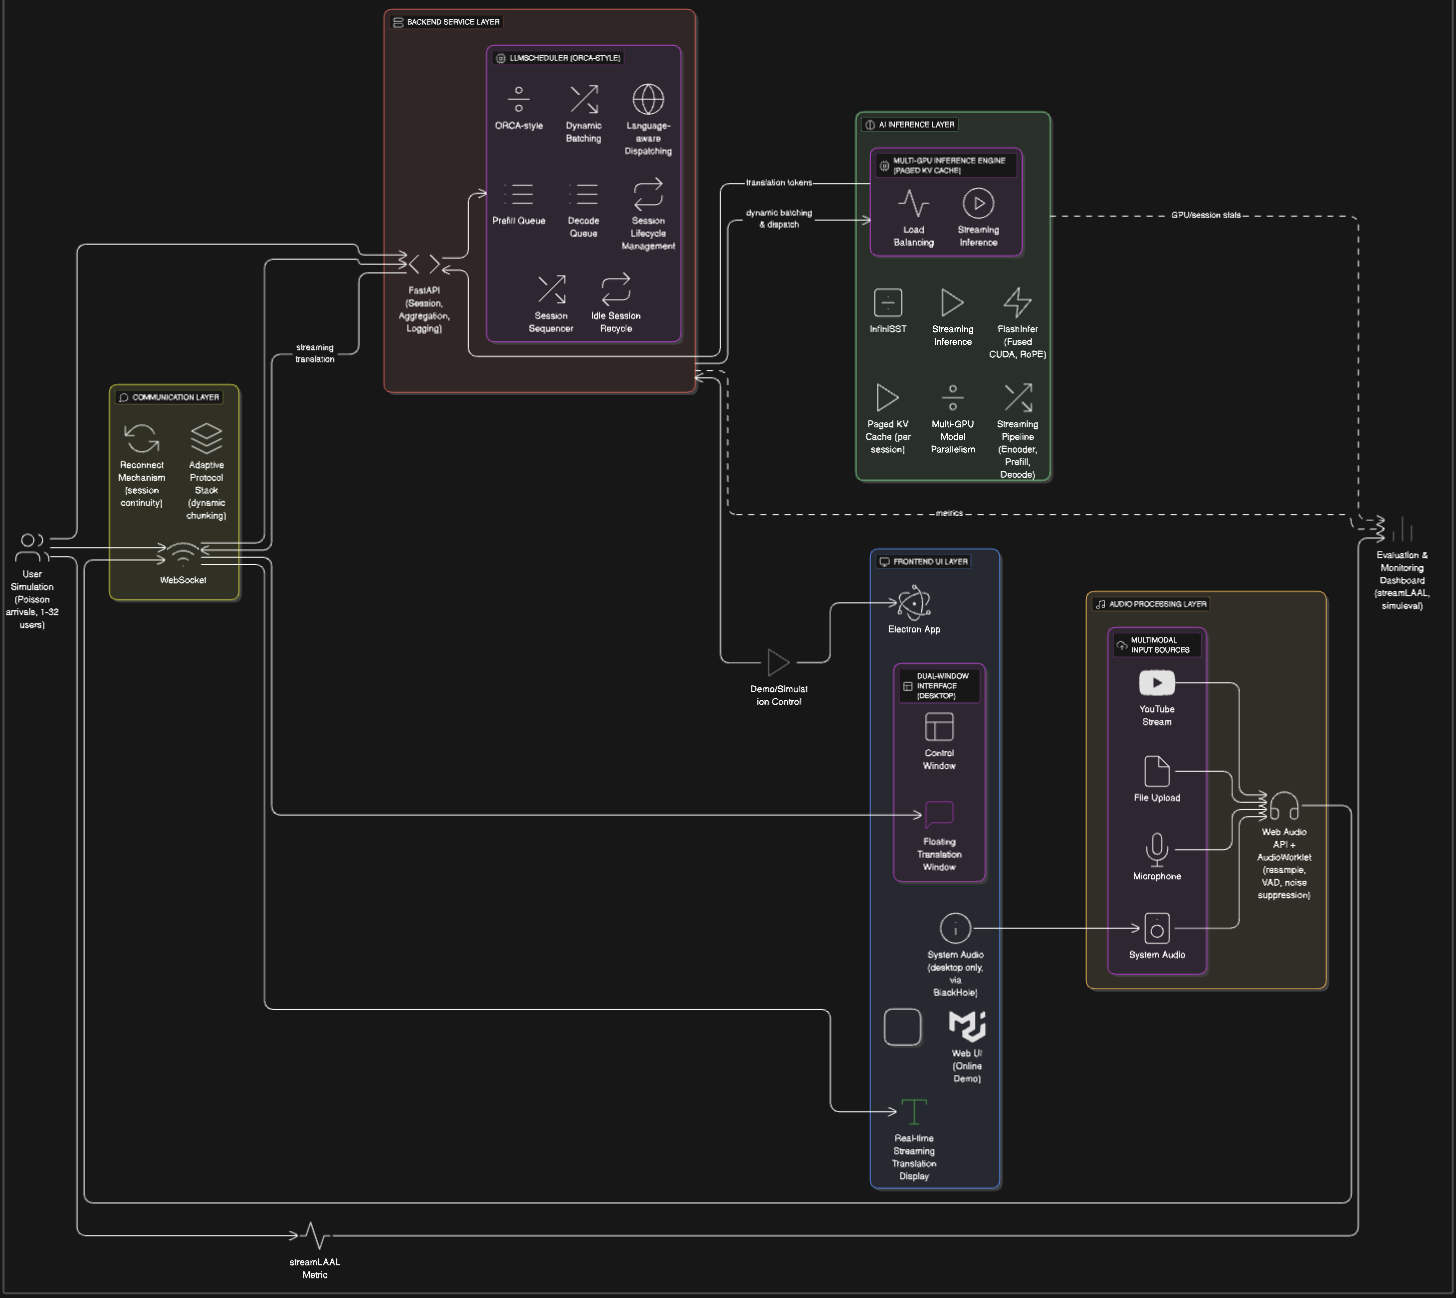
\includegraphics[width=1\linewidth]{architech.png}
    \caption{System Architecture}
    \label{fig:enter-label}
\end{figure}
The backend receives a batch of requests from the scheduler, performs one step of either prefilling or decoding for each request, and returns the updated requests to the scheduler.

\paragraph{Prefill}
Each prefill request consists of a speech input segment and the KV caches for both the speech encoder and the LLM. The request is first processed by the streaming speech encoder, which consumes the speech input and the encoder KV cache to produce speech features. These features are then passed to the LLM, along with its KV cache, to compute the logits of the first target token—thereby initiating the decoding process.

Since input sequence lengths vary across requests, we adopt the batching strategy from Orca~\cite{}, which concatenates inputs along the length dimension. Non-attention operations in both the speech encoder and LLM are position-wise and can thus be applied uniformly. For attention operations, we maintain a page table to support paged attention~\cite{} and utilize the FlashInfer~\cite{} library for efficient computation over variable-length sequences within the batch.

\paragraph{Beam Search Decoding} 
After the prefill stage, requests enter the decoding phase. We initialize the beam search state, which includes the number of unfinished beams, accumulated log probabilities, generated token sequences, and a buffer for completed beams. The KV cache is duplicated for each beam. Since we use paged attention, each request only stores pointers to the pages it references. To avoid physically copying memory, we duplicate only the page pointers (except for the final page, which may be modified) and increment the reference counter for each shared page.

In each decoding iteration, we perform one step of beam search and collect beams that have reached completion, storing their generated sequences and log probabilities. The sliding window and attention sink mechanisms are implemented by decrementing the reference counters of KV cache pages. When a page’s reference count reaches zero, it is returned to the pool of available pages.

Once all beams are completed, we select the one with the highest log probability as the final output. All KV cache pages used exclusively by non-selected beams are released.